\chapter{Clasificación con Deep Learning}\label{cap.clasificacion}
En este capítulo se expondrá el trabajo realizado para el entendimiento del problema de clasificación, mediante la elaboración de un componente en Python que permite la clasificación de dígitos del 0 al 9 en tiempo real, y la realización de un amplio estudio sobre las variantes posibles aplicadas a las redes entrenadas, utilizando la plataforma Caffe.\\
\section{Clasificador de dígitos}
Se ha desarrollado un componente en Pyhton para la clasificación de dígitos entre 0 y 9 en tiempo real, siendo necesario, previamente, un entendimiento de una primera red básica, utilizada por el mismo para la tarea. En esta sección se explicará el procedimiento seguido para el entendimiento de la red y el desarrollo del propio componente.\\
\subsection{Red básica}\label{sec.red}
La red que se empleará, está orientada a la clasificación de números utilizando, en el entrenamiento, la base de datos numérica MNIST, explicada en la Sección~\ref{sec.minst}.\\
Para realizar el entrenamiento de la red, Caffe proporciona tres archivos que se editarán para adaptar la red al problema que se abarque. A continuación, se explicará cada uno de esos archivos, siguiendo el orden que fue necesario hasta conseguir la red completamente entrenada.
\vspace{15pt}
\subsubsection{Definición de la red}
	Caffe utiliza el archivo 
	\textit{lenet\_train\_test.prototxt} para la especificación de todos los parámetros que son necesarios en el entrenamiento de la red, es decir, define las imágenes que se emplearán, la propia estructura de la red y la forma en la que se analizarán las imágenes proporcionadas, todo ello empleando diferentes capas (\textit{layers}).\\

	La primera línea de este documento es utilizada para indicar el nombre que se le quiere dar a la red.
	\vspace{10pt}
	\begin{lstlisting}[frame=single]
	name: "LeNet"
	\end{lstlisting}
	
	En concreto, esta red recibe el nombre de LeNet, un tipo de red que es conocida por un buen funcionamiento en las tareas de clasificiación de dígitos y que, por lo general, consta de una capa convolucional seguida por una capa de agrupamiento (\textit{pooling}), repetido dos veces y, finalmente, dos capas totalmente conectadas similares a las perceptrones multicapa convencionales. En el ejemplo de Caffe, la estructura habitual de la red LeNet se ve ligeramente modificada, ya que en lugar de emplear una función de activacion sigmoidal se utiliza una linear.\\

	Tras la definición del nombre se definen dos capas de datos, una de ellas correspondiente a los datos de entrenamiento de la red y, la otra, correspondiente a los datos que se utilizarán para realizar el test durante el entrenamiento para obtener datos de \textit{accuracy} y \textit{loss}.
	\vspace{10pt}
	\begin{lstlisting}[frame=single]
	layer {
		name: "mnist"
		type: "Data"
		top: "data"
		top: "label"
		include {phase: TRAIN}
		transform_param {scale: 0.00390625}
		data_param {
			source: "examples/mnist/mnist_train_lmdb"
			batch_size: 64
			backend: LMDB
		}
	}
	\end{lstlisting}
	
	Es importante que los parámetros de transformación, en este caso un factor de escala que establece el rango de la imagen en [0,1], sean los mismos en ambas fases, pues si se evaluase la red con una transformación de la imágen distinta a la aplicada en el entrenamiento los resultados obtenidos no serían reales.\\
	Se utilizará, por tanto, dos capas de datos que difieren en la fase en la que se utilizarán los datos, entrenamiento o evaluación de la red, el tamaño del lote, siendo 64 muestras para el entrenamiento y 100 para el test, y la ruta de la que se cogen los datos.\\

	A continuación, se comienzan a definir las capas del entrenamiento propiamente dicho. Se intercala una capa de convolución con una de agrupamiento y se repite dos veces.
	\vspace{10pt}
	\begin{lstlisting}[frame=single]
	layer {
		name: "conv1"
		type: "Convolution"
		bottom: "data"
		top: "conv1"
		param {lr_mult: 1}
		param {lr_mult: 2}
		convolution_param {
			num_output: 20
			kernel_size: 5
			stride: 1
			weight_filler {type: "xavier"}
			bias_filler {type: "constant"}
		}
	}	
	\end{lstlisting}

	En la capa de convolución, explicada en la Sección~\ref{sec.caffe}, se define que el tamaño del filtro será de 5x5 y que se obtendrán 20 salidas, en la segunda capa de convolución, sin embargo, se obtendrán 50 salidas. Además se define el algoritmo "Xavier" para la inicialización de los pesos, que determina automáticamente la escala de inicialización basada en el número de entradas y de las neuronas de salida, y la inicialización del \textit{bias} mediante una constante que por defecto es 0.
	\vspace{10pt}
	\begin{lstlisting}[frame=single]
	layer {
		name: "pool1"
		type: "Pooling"
		bottom: "conv1"
		top: "pool1"
		pooling_param {
			pool: MAX
			kernel_size: 2
			stride: 2
		}
	}	
	\end{lstlisting}
	
	La capa de agrupamiento, también explicada en la Sección~\ref{sec.caffe}, será alimentada por la capa de convolución anterior y alimentará a la siguiente en caso de que la haya. Se definen en ella un tamaño de filtro de 2x2, un intervalo de dos muestras entre cada aplicación del filtro, por lo que no hay solape, y el método del máximo para realizar el agrupamiento.\\

	Tras estas capas, se establecen dos capas completamente conectadas, \textit{InnerProduct}, separadas por la capa de activación, \textit{ReLu}, ambas explicadas en la Sección~\ref{sec.caffe}. 
	\vspace{10pt}
	\begin{lstlisting}[frame=single]
	layer {
		name: "ip1"
		type: "InnerProduct"
		bottom: "pool2"
		top: "ip1"
		param {lr_mult: 1}
		param {lr_mult: 2}
		inner_product_param {
			num_output: 500
			weight_filler {type: "xavier"}
			bias_filler {type: "constant"}
		}
	}	
	\end{lstlisting}
	
	\begin{lstlisting}[frame=single]
	layer {
		name: "relu1"
		type: "ReLU"
		bottom: "ip1"
		top: "ip1"
	}	
	\end{lstlisting}
	
	Las capas completamente conectadas se definen con, 500 salidas la primera de ellas, y tantas como clases se tengan en la segunda, en el caso concreto que se trata serán 10, correspondientes con los dígitos del 0 al 9.\\

	Para terminar la estructura de la red básica, Caffe permite la opción de añadir capas que muestren parámetros de evaluación de la red que se está entrenando. Para ello, en la Sección~\ref{sec.caffe}, se explicaron varias capas de \textit{Loss}, que serán empleadas en esta red para su evaluación, se deberán explicitar en este documento.
	\vspace{10pt}
	\begin{lstlisting}[frame=single]
	layer {
		name: "accuracy"
		type: "Accuracy"
		bottom: "ip2"
		bottom: "label"
		top: "accuracy"
		include {phase: TEST}
	}
	
	layer {
		name: "loss"
		type: "SoftmaxWithLoss"
		bottom: "ip2"
		bottom: "label"
		top: "loss"
	}	
	\end{lstlisting}
	
	Estas dos capas permiten obtener valores de precisión y pérdidas cada ciertas iteraciones, siendo marcado este valor en el siguiente documento.\\

	En la Figura~\ref{fig.redBasica} se puede observar un esquema de la estructura definida en este apartado, los valores de interés y cada una de las entradas y salidas de las capas.
	
	\begin{figure}[H]
		\begin{center}
			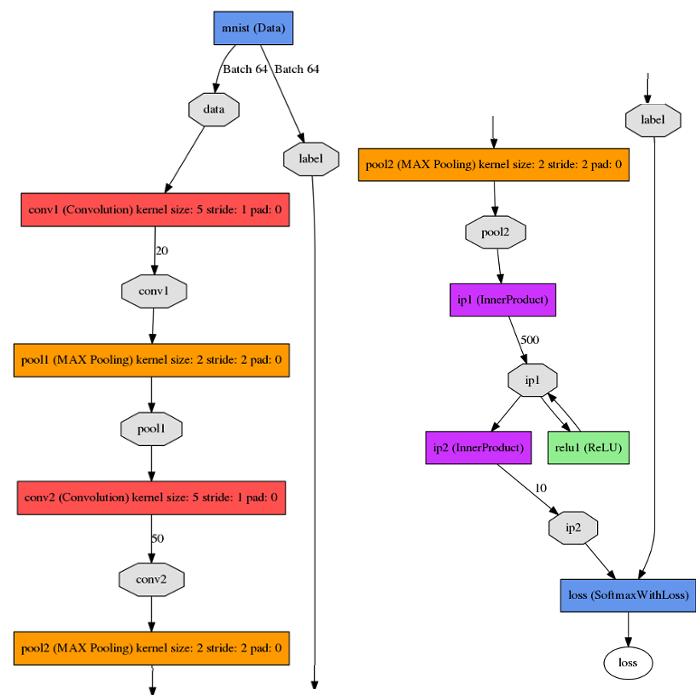
\includegraphics[width=0.8\textwidth]{figures/Original_net}
			\caption{Red básica LeNet MNIST}
			\label{fig.redBasica}
		\end{center}
	\end{figure}
	
	Para obtener la Figura~\ref{fig.redBasica}, se ha ejecutado un código proporcionado por la propia plataforma, que, mediante el archivo que define la estructura, explicado anteriormente, dibuja la red. Para ello se debe ejecutar el siguiente comando:
	\vspace{10pt}
	\begin{lstlisting}[frame=single]
	$ caffe/python/draw_net.py <netprototxt_filename> <out_img_filename>
	\end{lstlisting}
\subsubsection{Definición del solucionador}
	Para esta tarea se va a utilizar el archivo de Caffe \textit{lenet\_solver.prototxt}, que permitirá manejar parámetros del propio entrenamiento de la red.\\ 
	Se definen en él parámetros como la estructura de red que se utilizará, definida en el apartado anterior, y el número de iteraciones que se ejecutarán durante el entrenamiento de la red, cuya explicación se aportó en la Sección~\ref{sec.caffe}. Además, en ese mismo capítulo, se explican el resto de parámetros que se manejarán en este proyecto, como la evaluación de la red o las redes intermedias que se guardarán.
	\vspace{10pt}
	\begin{lstlisting}[frame=single]
	# The train/test net protocol buffer definition
	net: "examples/mnist/lenet_train_test.prototxt"
	# test_iter specifies how many forward passes the test should carry 
	# out.
	# In the case of MNIST, we have test batch size 100 and 100 test
	# iterations, covering the full 10,000 testing images.
	test_iter: 100
	# Carry out testing every 500 training iterations.
	test_interval: 500
	# The base learning rate, momentum and the weight decay of the network.
	base_lr: 0.01
	momentum: 0.9
	weight_decay: 0.0005
	# The learning rate policy
	lr_policy: "inv"
	gamma: 0.0001
	power: 0.75
	# Display every 100 iterations
	display: 100
	# The maximum number of iterations
	max_iter: 10000
	# snapshot intermediate results
	snapshot: 5000
	snapshot_prefix: "examples/mnist/lenet"
	# solver mode: CPU or GPU
	solver_mode: CPU	
	\end{lstlisting}
\subsubsection{Ejecución de la red}
	Una vez se han definido los parámetros adecuados para la red que se quiera entrenar, se ejecutarán los siguientes comandos, que comenzará con el entrenamiento de la red:
	\vspace{10pt}
	\begin{lstlisting}[frame=single]
	cd $CAFFE_ROOT
	./examples/mnist/train_lenet.sh	
	\end{lstlisting}
	
	El archivo que se ejecuta contiene información sobre qué solucionador se debe implementar y el modo de ejecución. Además es posible añadirle una línea que guardará un archivo con información de \textit{log} del proceso de entrenamiento.
	\vspace{10pt}
	\begin{lstlisting}[frame=single]
	#!/usr/bin/env sh
	set -e
	
	./build/tools/caffe train 
	  --solver=examples/mnist/lenet_solver_validation.prototxt 
	    2>&1 | tee /home/nuria/TFG/logs/RedBasica.log $@
	\end{lstlisting}
	
	\begin{figure}[H]
		\begin{center}
			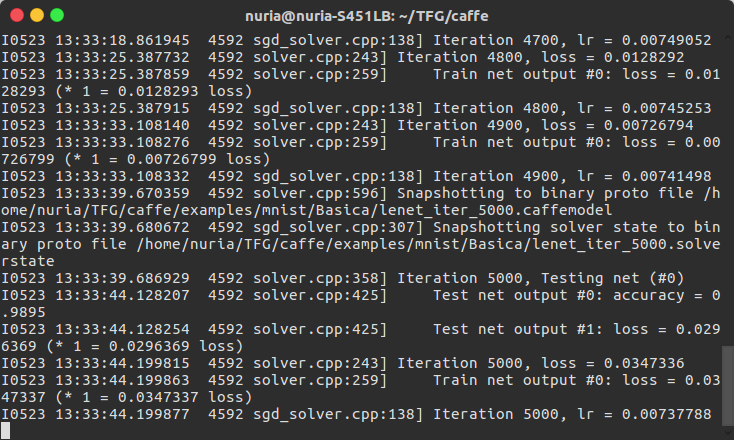
\includegraphics[width=0.8\textwidth]{figures/RedBasica5000}
			\caption{Ejecución de entrenamiento de red LeNet MNIST}
		\end{center}
	\end{figure}
	
	\begin{figure}[H]
		\begin{center}
			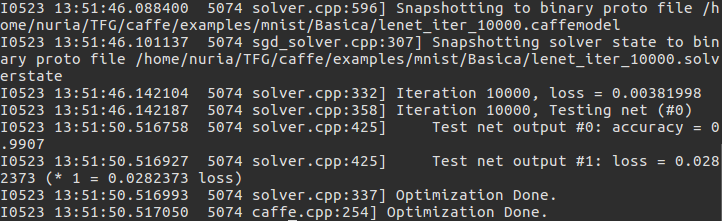
\includegraphics[width=0.8\textwidth]{figures/RedBasicaFin}
			\caption{Fin de entrenamiento de red LeNet MNIST}
			\label{fig.finEntrBas}
		\end{center}
	\end{figure}
	
	Tras terminar el entrenamiento, mostrado en la Figura~\ref{fig.finEntrBas}, se obtiene el archivo con la red neuronal entrenada, almacenado según la ruta que se indicó en el solucionador, que podrá ser utilizada en la herramienta que sea de interés.\\

	El archivo \textit{log} generado podrá ser visualizado mediante la ejecución del script \textit{plot\_learning\_curve.py} \footnote{https://github.com/adilmoujahid/deeplearning-cats-dogs-tutorial/blob/master/code/plot\_learning\_curve.py} de la siguiente forma:
	\vspace{10pt}
	\begin{lstlisting}[frame=single]
	python plot_learning_curve.py /home/nuria/TFG/logs/RedBasica.log 
	 RedBasicaLog.png
	\end{lstlisting}
	
	En la Figura~\ref{fig.Log} se puede observar el resultado final de la curva de aprendizaje, con valores de precisión y pérdidas, según lo explicado en la Sección~\ref{sec.caffe}, para la fase de evaluación, y en entrenamiento únicamente de pérdidas.
	
	\begin{figure}[H]
		\begin{center}
			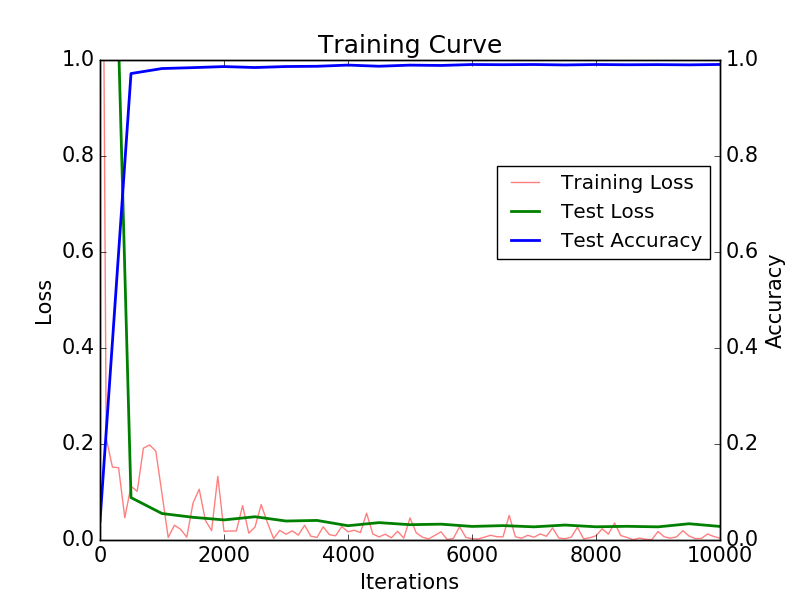
\includegraphics[width=0.5\textwidth]{figures/RedBasicaLog}
			\caption{Curva de aprendizaje Red Básica}
			\label{fig.Log}
		\end{center}
	\end{figure}

\subsection{Componente Python}
Se ha desarrollado un componente escrito en Python que, mediante la ayuda del \textit{Camera Server} de JdeRobot, comentado en la Sección~\ref{sec.jderobot},  y la red explicada en la Sección~\ref{sec.red}, es capaz de clasificar un dígito mostrado a la cámara, que se especificará en un archivo de configuración, en tiempo real, encendiendo una bombilla que se corresponde con el número obtenido.\\

Debido a la magnitud de la tarea a realizar, se optó por dividir el programa en dos hilos que serán explicados a continuación. Uno de ellos se encargará del aspecto gráfico de la aplicación, mostrando la imagen obtenida por la cámara, la imagen procesada para la clasificación, y la iluminación de la bombilla correspondiente. El segundo hilo, se encargará de gestionar la captación de la cámara, mediante la conexión con el componente \textit{Camera Server}, así como el proceso de clasificación, utilizando la red entrenada. Todo el código correspondiente a esta aplicación podrá ser encontrado en 
\subsubsection{Cámara}
El hilo fundamental de la aplicación, que se encargará de la lógica de la misma mediante la adquisición de la imagen y su posterior procesamiento, estará referenciado por el nombre \textit{Camera}.\\

Al comienzo de la ejecución se inicializa un objeto Cámara, mediante el constructor \textit{Camera()}, que será el encargado de gestionar las acciones anteriormente nombradas. En esta inicialización se indica qué cámara se va a utilizar, referenciada de manera externa mediante un archivo de configuración que se indicará en la ejecución de la aplicación. La línea que indica la cámara en este archivo es la siguiente:
\vspace{10pt}
\begin{lstlisting}[frame=single]
	Numberclassifier.Camera.Proxy=cameraA:default -h localhost -p 9999
\end{lstlisting}
Esta propiedad estará enlazada con el componente \textit{Camera Server} de JdeRobot que nos proporciona un servidor de imágenes mediante la cámara.\\

Otro aspecto importante que se maneja en la inicialización de la cámara es la especificación y carga de la red que se empleará para la clasificación. Este aspecto se realiza mediante las siguientes líneas:
\vspace{10pt}
\begin{lstlisting}[frame=single]
	model_file = '/home/nuria/TFG/caffe/examples/mnist/lenet.prototxt'
	pretrained_file = '/home/nuria/TFG/caffe/examples/mnist/Basica/
						/lenet_iter_10000.solverstate'
	self.net = caffe.Classifier(model_file, pretrained_file, 
									image_dims=(28, 28), raw_scale=255)
\end{lstlisting}
Mediante estas líneas se realizan las tres acciones necesarias para establecer la red que se utilizará. En primer lugar, se indica cuál será el modelo empleado para la clasificación. Este modelo es un archivo porporcionado Caffe de manera homóloga al \textit{lenet\_train\_test.prototxt}, con la excepción de que la capa de datos no recurre a archivos almacenados sino que utiliza imágenes que serán insertadas en la ejecución de la red. El resto de datos deben ser exáctamente iguales a la estructura de la red entrenada para que no se produzcan errores. En segundo lugar, se indica la red entrenada que se utilizará en la ejecución, el archivo obtenido al finalizar el entrenamiento según se indicó en la Sección~\ref{sec.red}. Por último, se crea la red ejecutable, es decir, se crea un objeto que será utilizado por la aplicación cada vez que se quiera realizar la clasificación. Para esta creación es necesario indicar, en primer lugar, que se trata de una red para la clasificación, y, además, introducir los parámetros del modelo, la red entrenada, las dimensiones de las imágenes, y la escala de los píxeles.\\

Además de las propiedades más importantes comentadas anteriormente, se definen también, funciones que serán importantes para la ejecución de la aplicación. Se establece una función \textit{update(self)}, que será llamada cada 150ms ya que, en el componente principal, se crea el hilo \textit{ThreadCamera(camera)} para obtener las imágenes de forma periódica y poder establecer un flujo de vídeo a tiempo real. Esta función, a su vez, necesita de otra, \textit{getImage(self)}, que obtiene la imagen, la redimensiona, y le aplica una transformación necesaria antes de introducirla en el proceso de clasificación, devolviendo un array con las dos imágenes, original y transformada. Para esa transformación se utiliza una tercera función de la cámara, \textit{trasformImage(self,img)}. En ella, se centra la imagen en un cuadrado, pues la captada es rectangular y la necesaria para introducir en la red cuadrada, se convierte a imagen de grises, se redimensiona al tamaño necesario para introducirla en la red (28x28), se le aplica un filtro gaussiano de 5x5 para reducir el ruido, y, por último, se le aplica el filtro de bordes de Sobel, en las dos direcciones (vertical y horizontal), y se realiza la suma de ambas para obtener la imagen final. Finalmente, se crea una función para realizar la clasificación de los dígitos:
\vspace{10pt}
\begin{lstlisting}[frame=single]
	def classification(self, img):
		self.net.blobs['data'].reshape(1,1,28,28)
		self.net.blobs['data'].data[...]=img * 0.00390625
		output = self.net.forward()
		digito = output['prob'].argmax()
		return digito
\end{lstlisting}
En primer lugar se asegura que las dimensiones del \textit{bolb} de datos sea de 28x28, valores establecidos para las imágenes. En el siguiente paso, se introduce a la red la imagen obtenida tras la transformación, aplicandole el factor de escala para que el intervalo de los píxeles esté entre 0 y 1, pues eso fue lo que se indicó en el aprendizaje. Posteriormente se ejecuta la red y se obtiene, como salida, una estructura que almacena, por un lado, la propiedad \textit{'prob'}, que se corresponde con un array que incluye las probabilidades de que la imagen introducida sea cada uno de los dígitos posibles, y, por otro, el tipo de datos que se almacena, en este caso \textit{float32}. Posteriormente, de ese array de probabilidades, se escoge el dígito cuya probabilidad es mayor, es decir, la clasificación realizada, y se devuelve.\\

Una vez establecida la lógica de la aplicación, se pasa a desarrollar el interfaz gráfico que permite al usuario visualizar, tanto las imágenes captadas y transformadas, como el resultado de la clasificación.
\subsubsection{GUI}
Para el aspecto gráfico de la aplicación, en el componente principal, se inicializará un objeto llamado \textit{window} mediante el constructor \textit{Gui()}, al que posteriormente se le vinculará la cámara mediante una función propia, \textit{window.setCamera(camera)}. Por último, al tratarse de un componente gráfico, será necesario indicar que se muestre mediante \textit{window.show()}. Al inicializar este objeto se crean todos los elementos gráficos que serán necesarios y que se modificarán posteriormente para conseguir el resultado deseado.\\

Al igual que en el caso de la cámara, se estabelcerá un hilo que permita aligerar la ejecución de la aplicación mediante \textit{ThreadGui(window)}, que establece el tiempo de actualización en 50ms. Debido al uso de este hilo, se crea en el objeto una función \textit{update()} que, en este caso, se encarga de obtener las imágenes original y transformada mediante la función \textit{getImage()} de la cámara, y adaptarlas para poder mostrarlas en las etiquetas definidas para cada una de ellas. Además, llama a otra función propia, \textit{lightON(out)}, que cambia el color del fondo del dígito que se haya clasificado, haciendo uso de la función de clasificación definida anteriormente en la cámara.\\

En la Figura~\ref{fig.gui} se puede observar el resultado gráfico de la aplicación. Al no tener detección, la ejecución de la clasificación es continua, por lo que, aunque no exista un dígito en la imagen, el componente decide constantemente un determinado dígito que considerará correcto, encendiendo la bombilla adecuada.\\

\begin{figure}[H]
	\begin{center}
		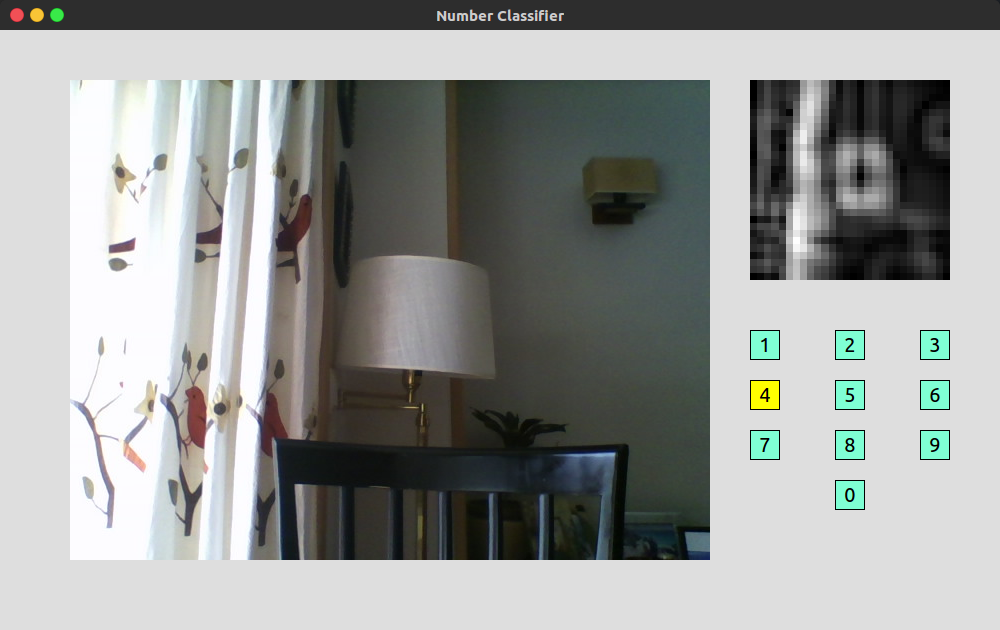
\includegraphics[width=0.8\textwidth]{figures/gui}
		\caption{Captura de componente gráfico de la aplicación}
		\label{fig.gui}
	\end{center}
\end{figure}

\subsubsection{Ejecución}
El proceso de ejecución del componente se divide en dos pasos. Por un lado, será necesaria la ejecución del servidor de imágenes, para lo que se utilizará el componente de JdeRobot. Por otro lado se debe lanzar el propio componente clasificador explicado anteriormente.\\

Para ejecutar el \textit{Camera Server}, se seguirán las instrucciones que aporta la plartaforma JdeRobot, utilizando el archivo de configuración que se facilita. Se utilizará el siguiente comando: 
\vspace{10pt}
\begin{lstlisting}[frame=single]
	cameraserver cameraserver.cfg
\end{lstlisting}

En el desarrollo de este trabajo, la propiedad de interés del archivo de configuración es \textit{CameraSrv.Camera.0.Uri}, que se centra en indicar la fuente de vídeo. Esta fuente puede ser un archivo de vídeo almacenado, para el que se emplearía la ruta del archivo en ese campo, la webcam del propio ordenador, para el que se utilizará el valor 0, u otra cámara externa, para la que se indicará el valor 1.\\

En la Sección~\ref{sec.droid} se comentó una aplicación que permitía utilizar la camara de un smartphone android como fuente de vídeo mediante una cámara externa. Para poder utilizar esta herramienta es necesario tener instalada el programa tanto en el dispositivo móvil a utilizar como en el propio ordenador, según se indica en las guía de la aplicación \footnote{https://www.dev47apps.com/droidcam/linuxx/}, y abrir la aplicación. Una vez abierta en ambos dispositivos, se debe conectar el USB del ordenador al móvil e indicar en la aplicación de escritorio que la conexión se hará vía USB. Se opta por la conexión USB, pues es más rápida y, por tanto, más adecuada a tiempo real. Una vez se han realizado las acciones anteriores se estable la conexión y se obtienen los resultados de las Figuras~\ref{fig.droidEsc}, en el ordenador, y ~\ref{fig.droidMov}, en el dispositivo.\\

\begin{figure}[H]
	\begin{center}
		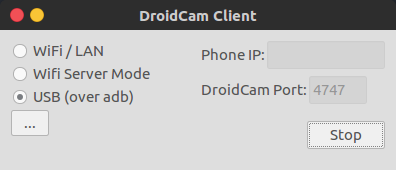
\includegraphics[width=0.4\textwidth]{figures/droidcamEscr}
		\caption{Captura de DroidCam en el ordenador}
		\label{fig.droidEsc}
	\end{center}
\end{figure}

\begin{figure}[H]
	\begin{center}
		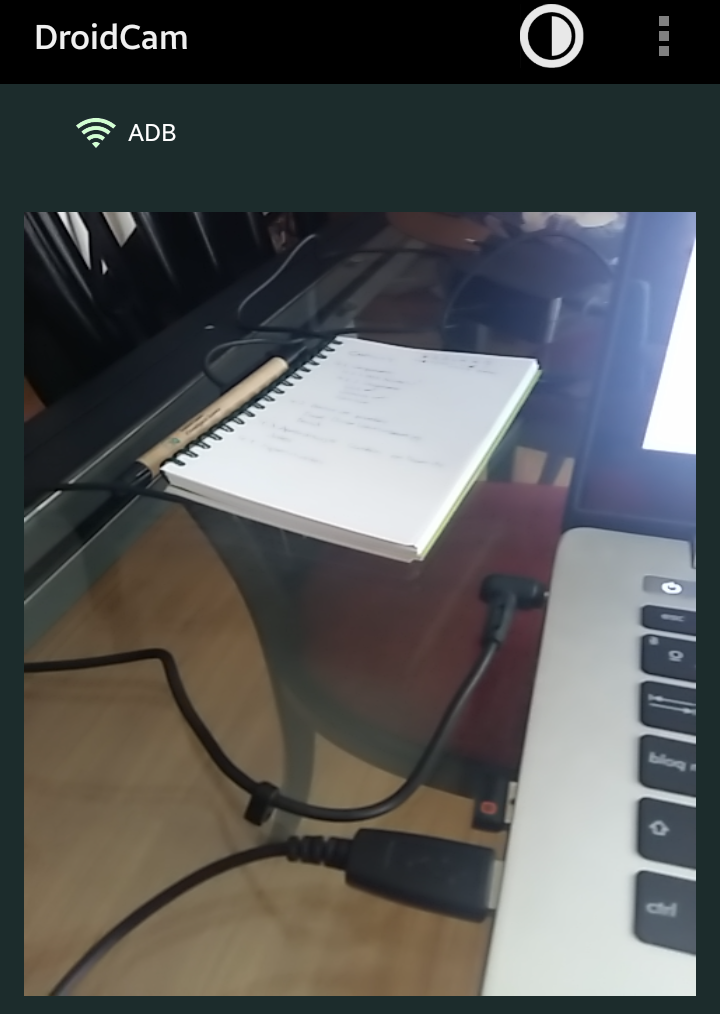
\includegraphics[width=0.3\textwidth]{figures/droidcamMov}
		\caption{Captura de DroidCam\\ 
			en el dispositivo móvil}
		\label{fig.droidMov}
	\end{center}
\end{figure}

Tras tener en funcionamiento el servidor de imágenes se debe proceder a la ejecución del componente clasificador. Para ello se ejecutará el siguiente comando:
\vspace{10pt}
\begin{lstlisting}[frame=single]
	python numberclassifier.py --Ice.Config=numberclassifier.cfg
\end{lstlisting}

El componente Python contiene los procedimientos indicados en las secciones anteriores, la creación del GUI, la cámara y el lanzamiento de los hilos correspondiente a cada uno. En el fichero de configuración se tiene una porpiedad que indica qué cámara utilizar. Es importante que el nombre de esta cámara se corresponda con el indicado en el fichero de configuración del servidor, de esta manera se establece la comunicación entre ambos componentes.\\

Finalmente, tras la ejecución, obtenemos el resultado del componente mostrado en la Figura~\ref{fig.componente1}, donde se aprecia el funcionamiento del mismo para un número sencillo y perfectamente definido.\\

Tras conseguir la aplicación del clasificador, se ha evaluado la red obtenida mediante un banco de pruebas, que será explicado a continuación y se ha procedido a la mejora de la misma.

\begin{figure}[H]
	\begin{center}
		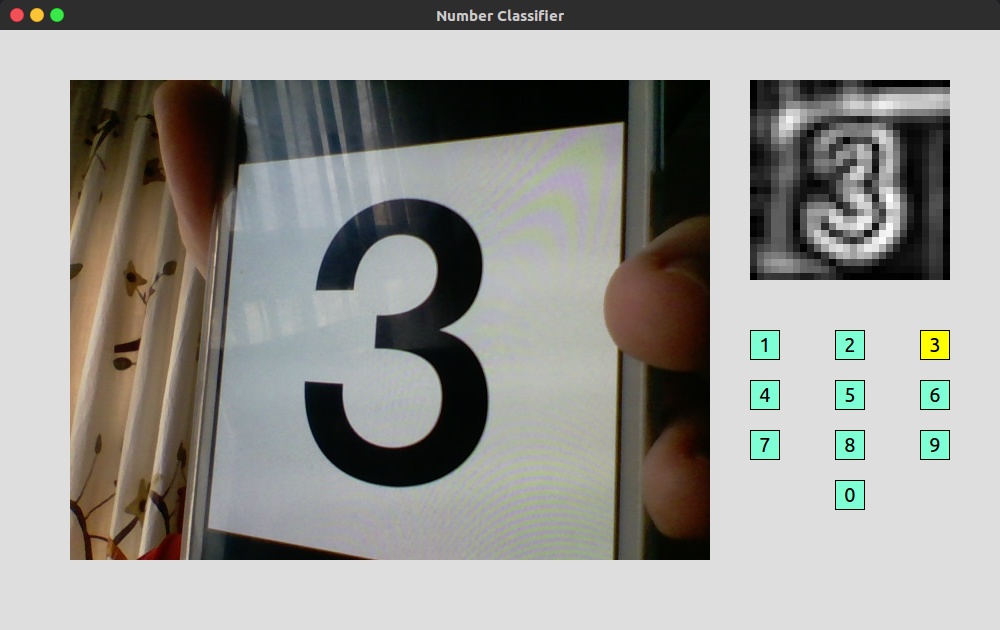
\includegraphics[width=0.5\textwidth]{figures/componente1}
		\caption{Captura del componente clasificador}
		\label{fig.componente1}
	\end{center}
\end{figure}

\section{Banco de pruebas}

\section{Efectos del aprendizaje}

\section{Experimentos}



